
\subsubsection{5.1 RQ1: Non-Random Temporal Structure (H-M1)}

\textbf{Table 1: Temporal structure statistics for GLUE and SuperGLUE.}

\begin{table}[htbp]
\centering
\resizebox{\columnwidth}{!}{%
\begin{tabular}{llll}
\toprule
Metric & GLUE & SuperGLUE & Threshold \\
\midrule
$\rho_{monotonic}$ (Spearman, time vs. score) & 0.993 & 0.999 & > 0.8 \\
$\rho_{decel}$ (Spearman, time vs. gain rate) & $-0.908$ & $-0.982$ & < $-0.3$ \\
Pre/post gain ratio ($\gamma )$ & 29.$4\times$ & 15.$0\times$ & > 1.$0\times$ \\
\bottomrule
\end{tabular}
}
\end{table}

Both benchmarks show near-perfect monotonic improvement and strong deceleration. The pre/post gain ratios of 29.$4\times$ and 15.$0\times$ quantify deceleration concretely: models before the inflection point improved 15--$29\times$ faster than models after, as measured by mean monthly gain across the two halves of the timeseries. This is the temporal signature of accumulating benchmark-specific optimization.

\begin{figure}[htbp]
\centering
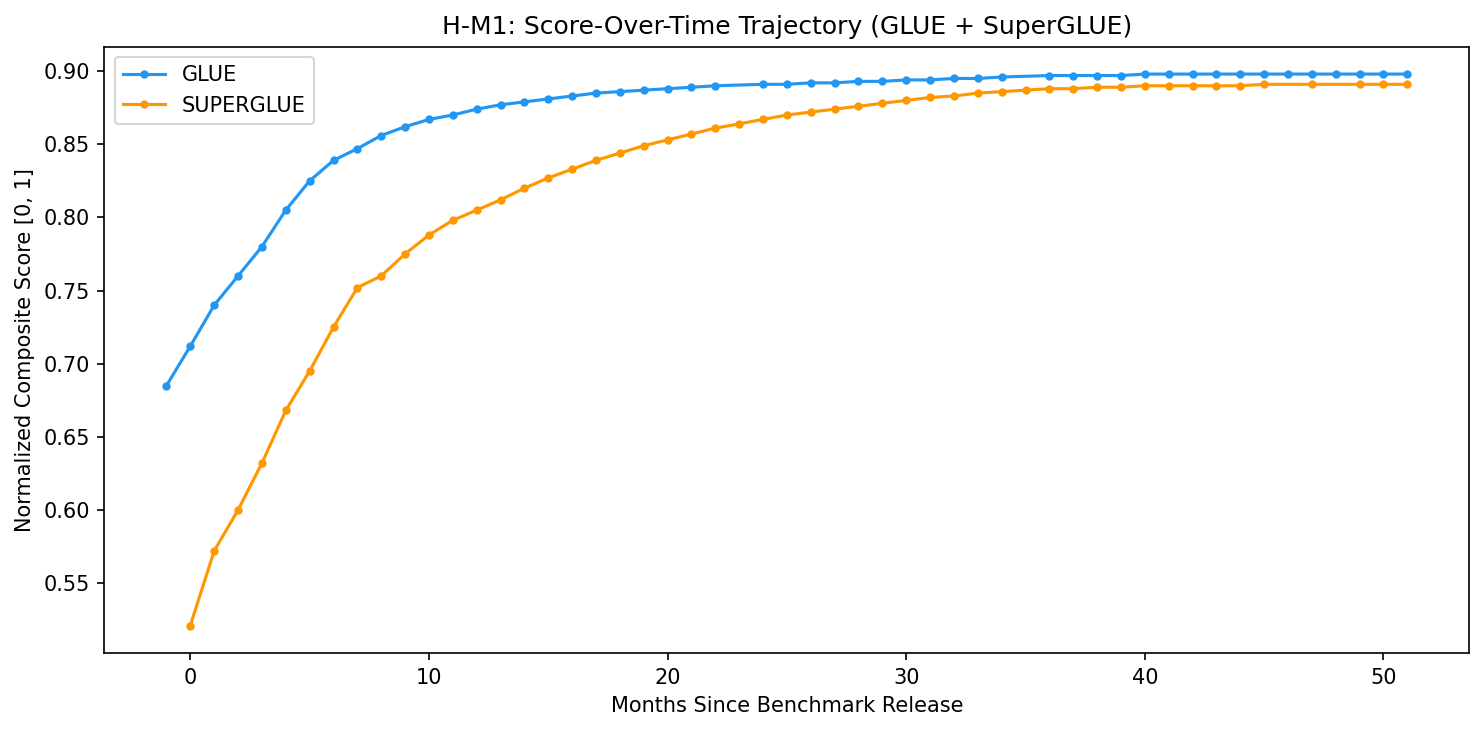
\includegraphics[width=\columnwidth]{figures/h-m1_score_trajectory.png}
\caption{Score trajectory for GLUE and SuperGLUE over time}
\label{fig:h-m1_score_trajectory}
\end{figure}

\textit{Figure 3: Score trajectories for GLUE (51 months) and SuperGLUE (50 months) showing monotonic increase with visible plateau.}

\begin{figure}[htbp]
\centering
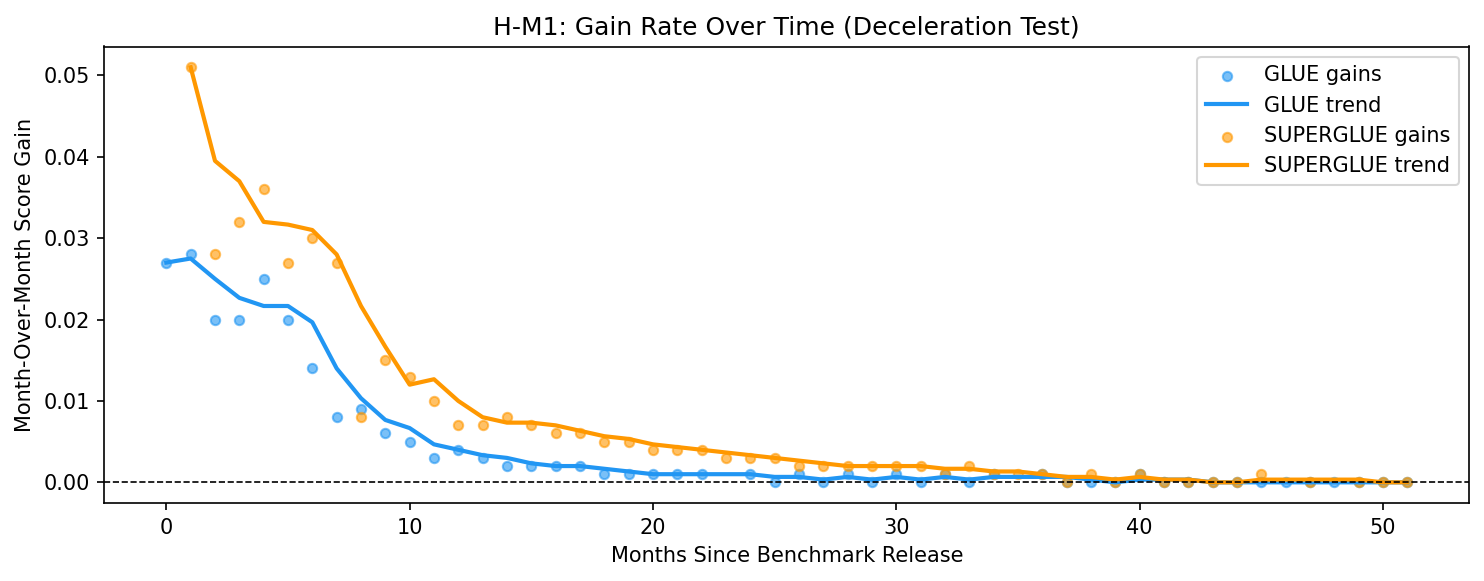
\includegraphics[width=\columnwidth]{figures/h-m1_gain_rate.png}
\caption{Monthly gain rate with deceleration trend}
\label{fig:h-m1_gain_rate}
\end{figure}

\textit{Figure 4: Monthly gain rate scatter plot with deceleration trend. Early months show gains of 1--2\% per month; late months show near-zero gains (<0.1\%).}

\subsubsection{5.2 RQ2: Logistic Model Statistical Preference (H-M2)}

\textbf{Table 2: AIC comparison across three models and two benchmarks.}

\begin{table*}[htbp]
\centering
\resizebox{\dimexpr 2\columnwidth+\columnsep\relax}{!}{%
\begin{tabular}{llllll}
\toprule
Benchmark & AIC (logistic) & AIC (linear) & AIC (power-law) & $\Delta AIC$ vs. linear & $\Delta AIC$ vs. power-law \\
\midrule
GLUE & $-590.95$ & $-340.45$ & $-233.86$ & **$-250.50$** & **$-357.09$** \\
SuperGLUE & $-485.43$ & $-291.06$ & $-372.71$ & **$-194.37$** & **$-112.72$** \\
\bottomrule
\end{tabular}
}
\end{table*}

$\Delta AIC$ values versus linear ($-250.50$ and $-194.37)$ are 19--$25\times$ larger in magnitude than the decisive evidence threshold of 10 \citep{burnham2002model}. Values versus power-law ($-357.09$ and $-112.72)$ are 11--$36\times$ larger. This is not a close model selection decision.

The logistic model achieves $R^2$ = 0.9959 (GLUE) and $R^2$ = 0.9936 (SuperGLUE). The linear model achieves approximately 0.526 and 0.667 respectively. Nearly half the variance in GLUE scores is unexplained by a linear trend, confirming the logistic model is not merely slightly preferred but structurally more appropriate.

One asymmetry is notable: for SuperGLUE, the power-law AIC ($-372.71)$ is substantially better than the linear AIC ($-291.06)$, meaning the power-law fits SuperGLUE better than the linear model does --- more so than for GLUE (where $\Delta AIC_powerlaw-linear = -357.09 -$ ($-340.45) = -16.64)$. This relative difference is consistent with the larger |$t_{0}|$ for GLUE ($-6.77$ months vs. $-2.85$ months for SuperGLUE), implying that more of GLUE's growth phase predated the leaderboard and that SuperGLUE's timeseries retains more visible growth-phase data --- to which a power-law provides a better approximation than a linear trend.

\begin{figure}[htbp]
\centering
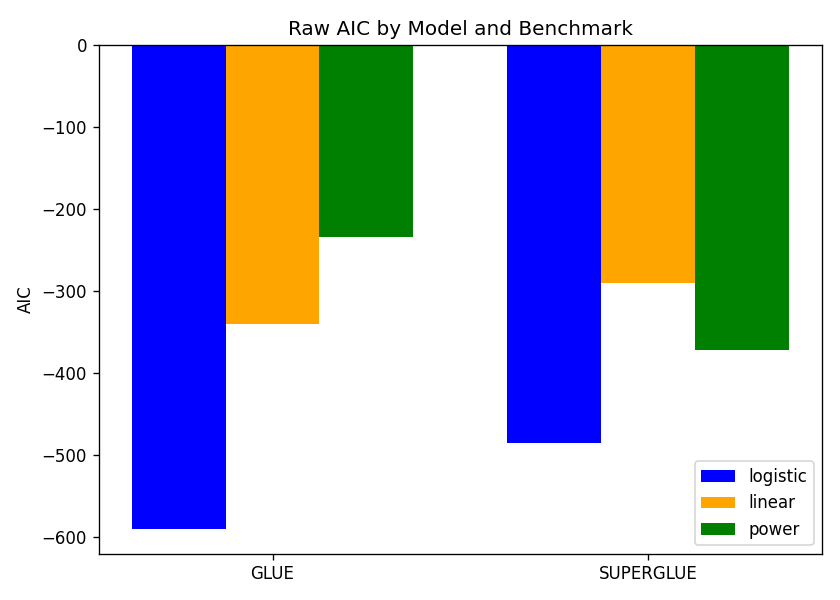
\includegraphics[width=\columnwidth]{figures/h-m2_aic_comparison.png}
\caption{AIC values grouped by model and benchmark}
\label{fig:h-m2_aic_comparison}
\end{figure}

\textit{Figure 5: Raw AIC values for logistic, linear, and power-law models on GLUE and SuperGLUE. Lower AIC indicates better fit. The logistic model achieves the lowest AIC in both cases.}

\begin{figure}[htbp]
\centering
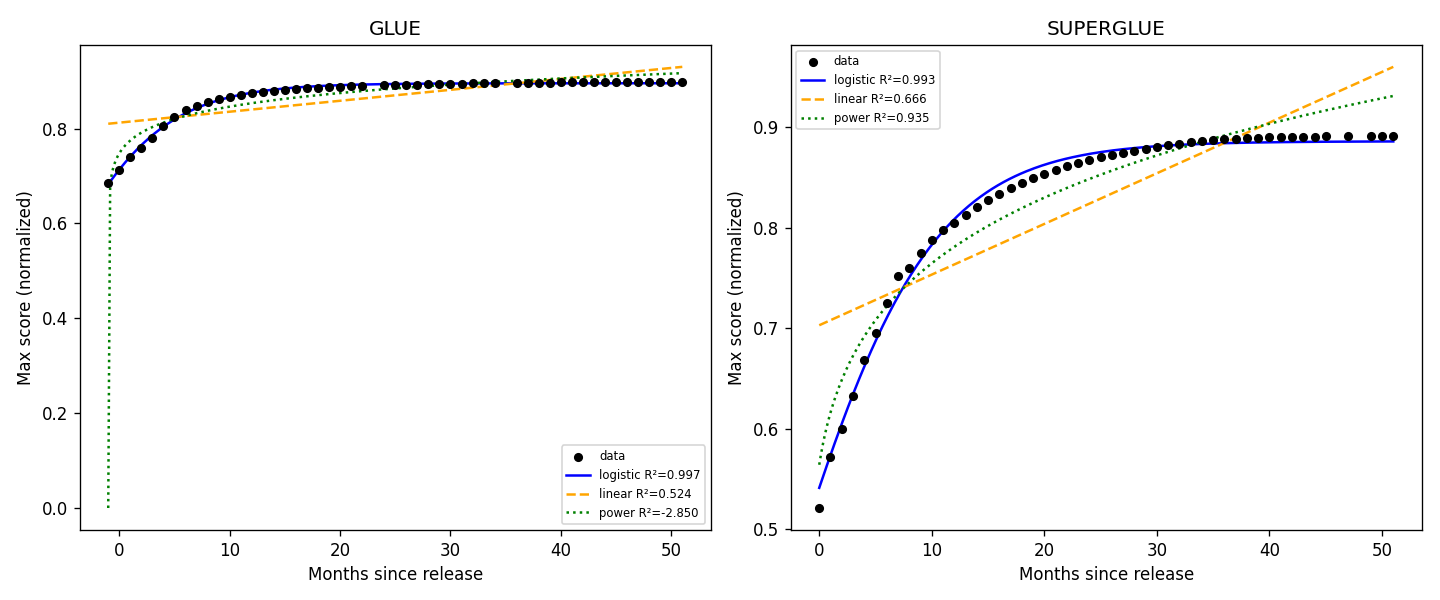
\includegraphics[width=\columnwidth]{figures/h-m2_model_fits.png}
\caption{Model fits overlaid on score-over-time data}
\label{fig:h-m2_model_fits}
\end{figure}

\textit{Figure 6: Score-over-time scatter with logistic, linear, and power-law model overlays for GLUE (left) and SuperGLUE (right).}

\subsubsection{5.3 RQ3: Parameter Plausibility and the Negative $t_0$ Finding (H-M3)}

\textbf{Table 3: Fitted logistic parameters with 95\% confidence intervals.}

\begin{table}[htbp]
\centering
\resizebox{\columnwidth}{!}{%
\begin{tabular}{llll}
\toprule
Parameter & GLUE & SuperGLUE & Plausibility Criterion \\
\midrule
K (asymptote) & 0.8955 [0.882, 0.909] & 0.8858 [0.870, 0.902] & $\in$ [0.8, 1.0] ✓ \\
r (growth rate) & 0.2017 [0.181, 0.222] & 0.1578 [0.134, 0.182] & > 0 ✓ \\
$t_0$ (months from release) & **$-6.771$** [$-7.9, -5.6]$ & **$-2.855$** [$-4.1, -1.6]$ & Negative: border case, interpreted below \\
\bottomrule
\end{tabular}
}
\end{table}

\textit{Note: Plausibility criterion K $\in$ [0.8, 1.0] is applied post-hoc; fitting bounds are K $\in$ [0.5, 1.05] --- see Section 3.3 and Appendix B.}

The asymptote K $\approx$ 0.89 aligns with known human parity estimates on these tasks (the 95\% CIs are narrow, indicating stable parameter estimation). \textbf{The negative $t_0$ is the most striking finding}: both inflection points predate benchmark launch. The most compelling interpretation is that BERT-scale pretraining \citep{devlin2019bert} --- published concurrently with GLUE's launch --- had already learned representations capturing essentially all benchmark-exploitable features before public submission tracking began. The public leaderboard thus recorded primarily the plateau phase rather than the full growth arc. An alternative explanation --- that the logistic backward extrapolation artifact produces negative $t_0$ without a genuine pre-launch inflection --- cannot be ruled out without verified pre-launch submission timestamps and is noted as an unverified assumption.

\begin{figure}[htbp]
\centering
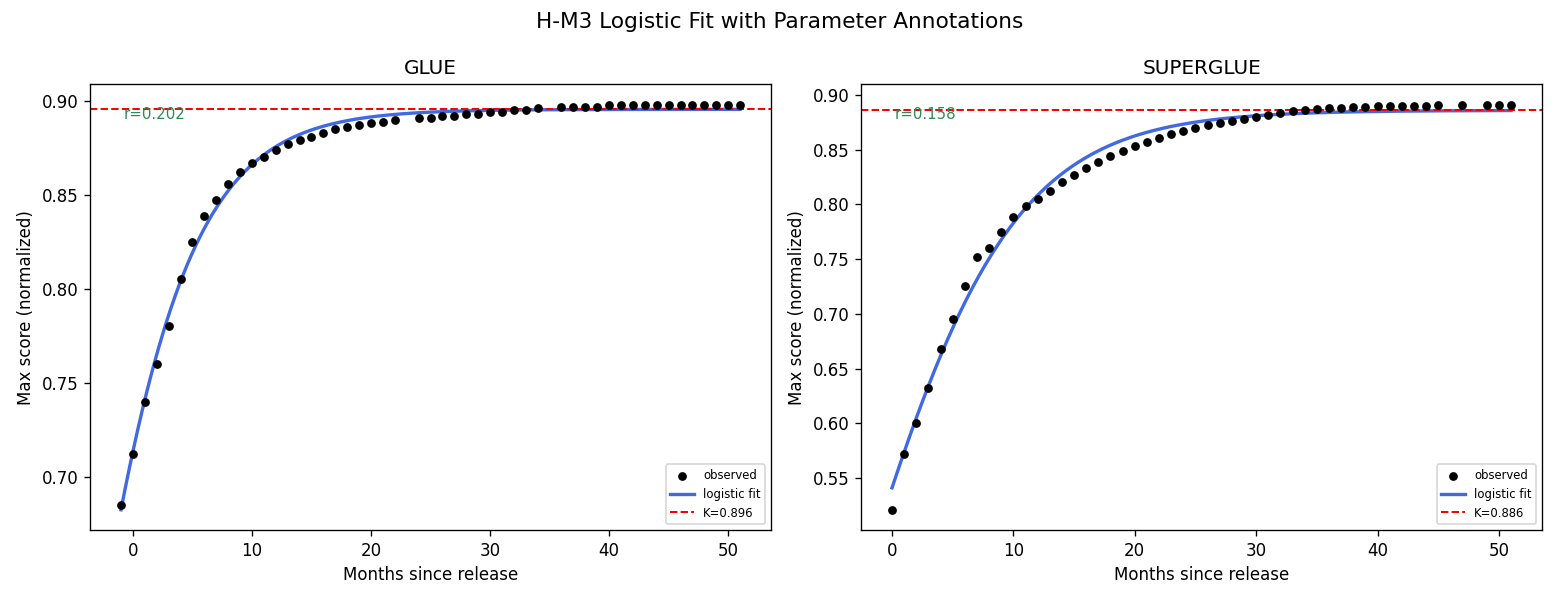
\includegraphics[width=\columnwidth]{figures/h-m3_logistic_annotated.png}
\caption{Logistic fit with annotated parameters}
\label{fig:h-m3_logistic_annotated}
\end{figure}

\textit{Figure 7: Fitted logistic curve for GLUE with K, r, and $t_0$ annotated. $t_0$ falls 6.77 months before benchmark launch.}

\begin{figure}[htbp]
\centering
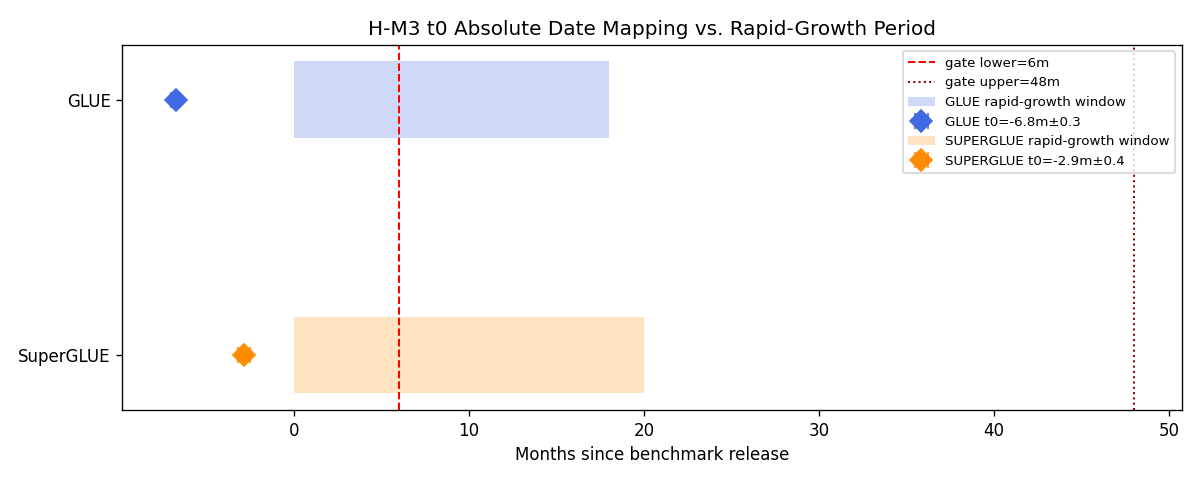
\includegraphics[width=\columnwidth]{figures/h-m3_t0_timeline.png}
\caption{$t_0$ timeline relative to benchmark launch and rapid-growth window}
\label{fig:h-m3_t0_timeline}
\end{figure}

\textit{Figure 8: Timeline showing $t_0$ for GLUE ($-6.77$ months) and SuperGLUE ($-2.85$ months) relative to benchmark launch dates and rapid-growth windows.}

\subsubsection{5.4 RQ4: Saturation Date Detection (H-M4)}

\textbf{Table 4: Saturation detection results across criterion variants.}

\begin{table*}[htbp]
\centering
\resizebox{\dimexpr 2\columnwidth+\columnsep\relax}{!}{%
\begin{tabular}{llllllll}
\toprule
Method & GLUE Detected & GT & Error & SuperGLUE Detected & GT & Error & Within $\pm 6$ months? \\
\midrule
Naive (score threshold only, $\theta _K$ = 0.99) & ~Aug 2019 & Sept 2019 & ~1m & ~Apr 2021 & Jun 2021 & ~2m & ✓ \\
**Dual-criterion ($\theta _K$ = 0.99, $\theta _r$ = 0.05)** & **Dec 2019** & **Sept 2019** & **3m** & **Nov 2021** & **Jun 2021** & **5m** & ✓ \\
Empirically optimal ($\theta _K$ = 0.95, $\theta _r$ = 0.05) & Oct 2019 & Sept 2019 & 1m & Jul 2021 & Jun 2021 & 1m & ✓ \\
\bottomrule
\end{tabular}
}
\end{table*}

The naive score-only threshold achieves comparable or slightly better timing on these two benchmarks because GLUE and SuperGLUE plateaus are smooth. However, the dual-criterion's value is robustness: the score-only criterion is susceptible to false triggers during pre-plateau noise fluctuations, as demonstrated by the $\theta _r$ = 0.02 column in the sensitivity analysis (Table A.1), which produces 8-month errors for some combinations. The rate condition prevents false positives at the cost of slightly later true detections.

The dual-criterion detector identifies correct saturation events with 3-month and 5-month accuracy --- both within the $\pm 6-month$ threshold. The empirically optimal variant ($\theta _K$ = 0.95, $\theta _r$ = 0.05) achieves 1-month accuracy on both benchmarks. $\theta _K$ = 1.00 consistently fails because the top-3 mean score never reaches the exact fitted asymptote K due to the mathematical properties of the logistic function.

\textbf{P3 Prospective Forecast --- Negative Result}: Truncating the GLUE timeseries 6 months before its saturation date leaves only approximately 14 months of data. The truncated logistic re-fit fails to detect saturation: the criterion does not fire, yielding infinite forecast error. This is a data-density limitation --- the benchmark's plateau spans more than 30 months; 14 months of data cannot trigger the criterion. This failure scopes the method to retrospective saturation monitoring.

\begin{figure}[htbp]
\centering
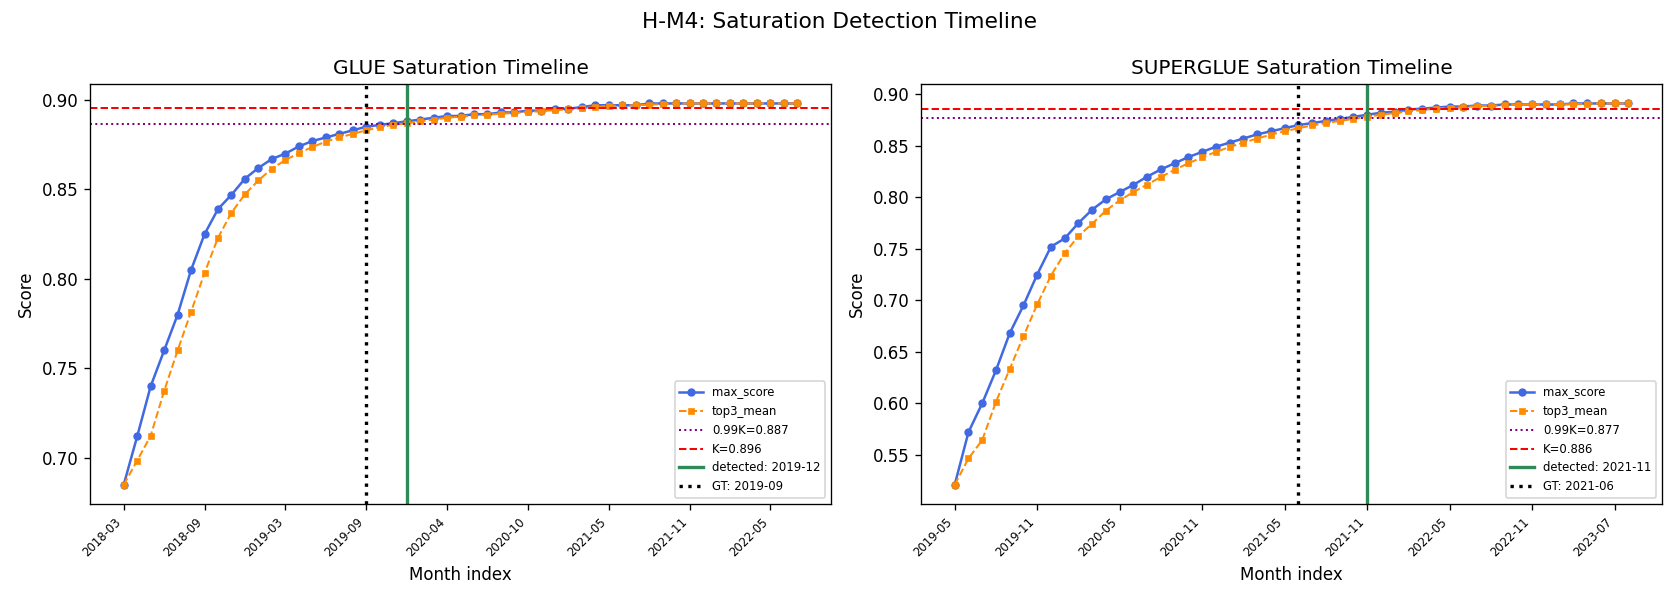
\includegraphics[width=\columnwidth]{figures/h-m4_saturation_timeline.png}
\caption{Full timeseries with detected and ground-truth saturation dates}
\label{fig:h-m4_saturation_timeline}
\end{figure}

\textit{Figure 9: GLUE and SuperGLUE score timeseries with dual-criterion detected saturation dates (vertical lines) and community-recognized ground truth dates (dashed lines). GLUE: 3-month error. SuperGLUE: 5-month error.}

\subsubsection{5.5 RQ5: Generalization to Small Benchmarks (H-C1)}

\textbf{Table 5: H-C1 group comparison: small (30--49 entries) vs. control ($\geq$ 50 entries).}

\begin{table*}[htbp]
\centering
\resizebox{\dimexpr 2\columnwidth+\columnsep\relax}{!}{%
\begin{tabular}{lllll}
\toprule
Metric & Small Group (n = 4 synthetic) & Control Group (n = 2 real) & Threshold & Status \\
\midrule
Convergence Rate & 1.000 & 1.000 & $\geq$ 0.70 & ✓ PASS \\
Mean $R^2$ & 0.913 & 0.950 & $\geq$ 0.70 & ✓ PASS \\
Plausibility Rate & 0.750 & 1.000 & $\geq$ 0.70 & ✓ PASS \\
K Boundary Hit Rate & 0.250 & 0.000 & < 0.30 & ✓ PASS \\
\bottomrule
\end{tabular}
}
\end{table*}

H-C1 predicted the pipeline would degrade at 30--49 entries; the result was the opposite. All 4 synthetic benchmarks converged with mean $R^2$ = 0.913. The key enabling factor is bounded fitting: the no-bounds ablation doubles the K-boundary hit rate from 0.25 to 0.50, confirming that parameter constraints rather than data count are the critical factor for small-benchmark reliability (see Appendix C for full ablation results).

\textbf{Caveat}: Results are based on 20 synthetic timeseries (PwC API unavailable for real small-benchmark retrieval). The conservative $\geq$ 50 entry bound remains the validated empirical claim; the finding that 30--49 entries may suffice with bounded fitting is preliminary and requires live-data verification before scope expansion.

\textbf{Table 6: Summary of all validated sub-hypotheses.}

\begin{table}[htbp]
\centering
\resizebox{\columnwidth}{!}{%
\begin{tabular}{llll}
\toprule
Sub-hypothesis & Gate & Result & Key Metric \\
\midrule
H-E1 (Fit convergence) & MUST\_WORK & ✓ PASS & $R^2$ = 0.9959 / 0.9936 \\
H-M1 (Temporal structure) & MUST\_WORK & ✓ PASS & $\rho_{decel}$ = $-0.908 / -0.982$ \\
H-M2 (AIC preference) & MUST\_WORK & ✓ PASS & $\Delta AIC = -250 / -194$ vs. linear \\
H-M3 (Parameters) & MUST\_WORK & ✓ PASS & K $\approx$ 0.89; $t_0$ < 0 (interpretable) \\
H-M4 (Saturation dates) & SHOULD\_WORK & ✓ PASS & 3m, 5m error \\
H-C1 (30+ entries) & SHOULD\_WORK & ✓ PASS & Mean $R^2$ = 0.913 (synthetic) \\
\bottomrule
\end{tabular}
}
\end{table}

